\section{La piattaforma Atlas e l'algoritmo Mindpulse}
{\bf Vibre}, un'azienda nel territorio cesenate, si prepone come mission e come modello di business l'idea di rendere facilmente fruibile ad un vasto pubblico il valore informativo che le neuroscienze hanno da offrire attraverso delle interfacce neurali passive, facili da usare e facilmente scalabili.\newline
Per ottenere questo risultato Vibre ha lavorato negli anni alla piattaforma {\bf Atlas}, un \emph{servizio cloud-based preposto all'elaborazione di segnali EEG} (ottenuti attraverso i dispositivi \emph{Muse} \cite{muse} (\emph{figura 1.3})) al fine di ottenere delle metriche che descrivano lo stato cognitivo di un soggetto.\newline
\begin{figure}[H]
  \centering
  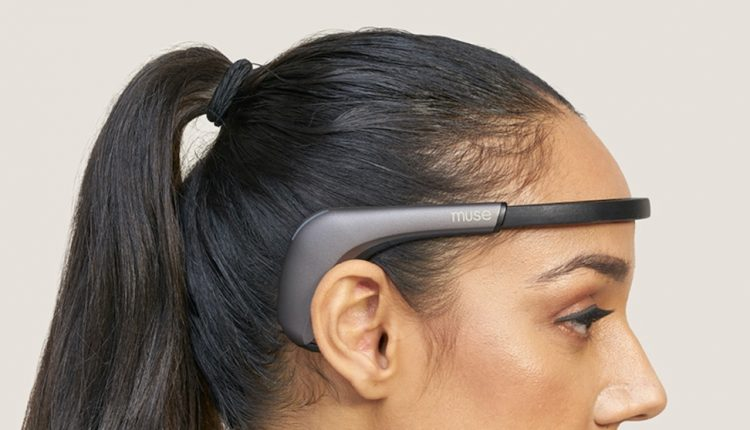
\includegraphics[width=1.0\textwidth]{img/muse2.jpg}
  \caption{Dispositivo Muse2 \cite{immagine_muse}}
\end{figure}
\vspace{8mm}
Atlas (\emph{figura 1.4}) è descrivibile ad alto livello come un sistema composto da:
\begin{itemize}
  \item \textbf{Algorithm packages}\\
  L'insieme dei tre algoritmi Python sviluppati da Vibre capaci di estrapolare metriche cognitive elaborando segnali EEG:
  \begin{itemize}
    \item \emph{MindFeel}
    \item \emph{MindPulse}
    \item \emph{MindPrint}
  \end{itemize}
  \item \textbf{Neuroserver}\\
  Un server REST che espone gli endpoint dei tre algoritmi ai servizi che ne richiedono la computazione.
\end{itemize}
\begin{figure}[H]
  \centering
  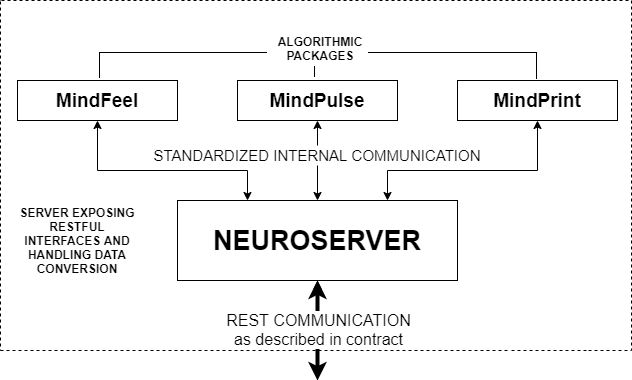
\includegraphics[width=0.90\textwidth]{img/atlas.png}
  \caption{Vista ad alto livello della piattaforma Atlas}
\end{figure}
Un servizio erogato ad un'azienda dunque, ottenendo dati dal dispositivo Muse, invierà i segnali EEG a Neuroserver che si occuperà di consegnarli all'algoritmo giusto al fine di ottenere dati rilevanti per il servizio in uso.\newline

\noindent Ai fini di questa tesi discuteremo brevemente e ad alto livello l'algoritmo {\bf MindPulse}, così da meglio comprendere il progetto svolto.\newline
MindPulse, attraverso della variazione delle onde Alpha, Beta, Theta e Delta emesse dal cervello e rilevate dal dispositivo Muse, è in grado di determinare delle metriche di facile interpretazione che descrivono il benessere cognitivo di un individuo.\newline
In modo particolare l'algoritmo (dopo aver effettuato una calibrazione sul soggetto) permette di comprendere:
\begin{itemize}
  \item \emph{Carico cognitivo (sezione 1.1)}\\
  Descrive il carico di lavoro compiuto al momento da un individuo, andando da uno stato di massimo relax fino ad uno stato di massimo impegno.
  \item \emph{Affaticamento mentale (sezione 1.1)}\\
  Descrive l'affaticamento mentale accumulato nel tempo (ad esempio dopo una intensa mattinata di lavoro un individuo risulterà maggiormente affaticato ed avrà a disposizione meno "risorse mentali").
\end{itemize}
Questo algoritmo è dunque alla base del {\emph macro-progetto} all'interno del quale si inserisce questa tesi: {\bf NeuroFrame}.
